\documentclass[8pt,a4paper,compress]{beamer}

\usepackage{/home/siyer/lib/slides}

\title{Compilation}
\date{}

\begin{document}
\begin{frame}
\vfill
\titlepage
\end{frame}

\begin{frame}
\frametitle{Outline}
\tableofcontents
\end{frame}

\section{Compilers}
\begin{frame}[fragile]
\pause

A compiler is a program that translates a source program written in a high-level programming language such as Java, C\lstinline{#} or C, into a target program in a lower level language such as machine code

\begin{center}
\visible<2->{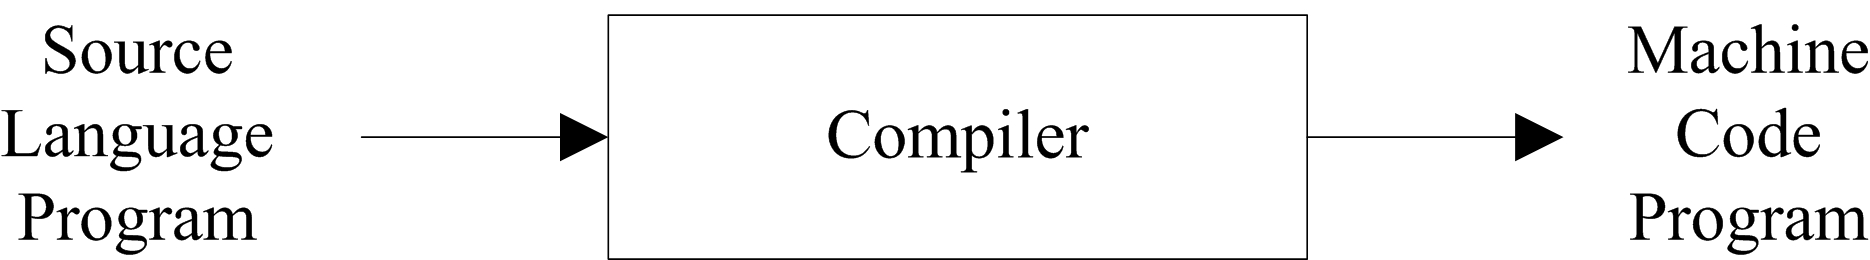
\includegraphics[scale=0.6]{{figures/figure01.01}.jpg}}
\end{center}

\pause
\bigskip

A programming language is an artificial language in which a programmer writes a program to control the behavior of a computer

\pause
\bigskip

Like a natural language, in a programming language, one describes
\begin{itemize}
\item The tokens (aka lexemes)

\item The syntax of programs and language constructs such as classes, methods, statements and expressions

\item The meaning (aka semantics) of the various constructs
\end{itemize}
\end{frame}

\begin{frame}[fragile]
\pause

A computer's machine language (ie, its instruction set) is designed so as to be easily interpreted by the computer itself

\pause
\bigskip

A machine's instruction set and its behavior is often referred to as its architecture

\pause
\bigskip

Examples of architectures
\begin{itemize}
\item Intel i386, a complex instruction set computer (CISC) with powerful and complex instructions

\item MIPS, as a reduced instruction set computer (RISC) with relatively simple instructions

\item Java Virtual Machine (JVM), a virtual machine not necessarily implemented in hardware
\end{itemize}

\pause
\bigskip

Traditionally, a compiler analyzes the input program to produce (or synthesize) the output program
\begin{itemize}
\item mapping names to memory addresses, stack frame offsets, and registers,

\item generating a linear sequence of machine code instructions, and

\item detecting any errors in the program that can be detected in compilation
\end{itemize}
\end{frame}

\begin{frame}[fragile]
\pause

An interpreter executes a high-level language program directly, ie, the high-level program is first loaded into the interpreter, and then executed

\begin{center}
\visible<2->{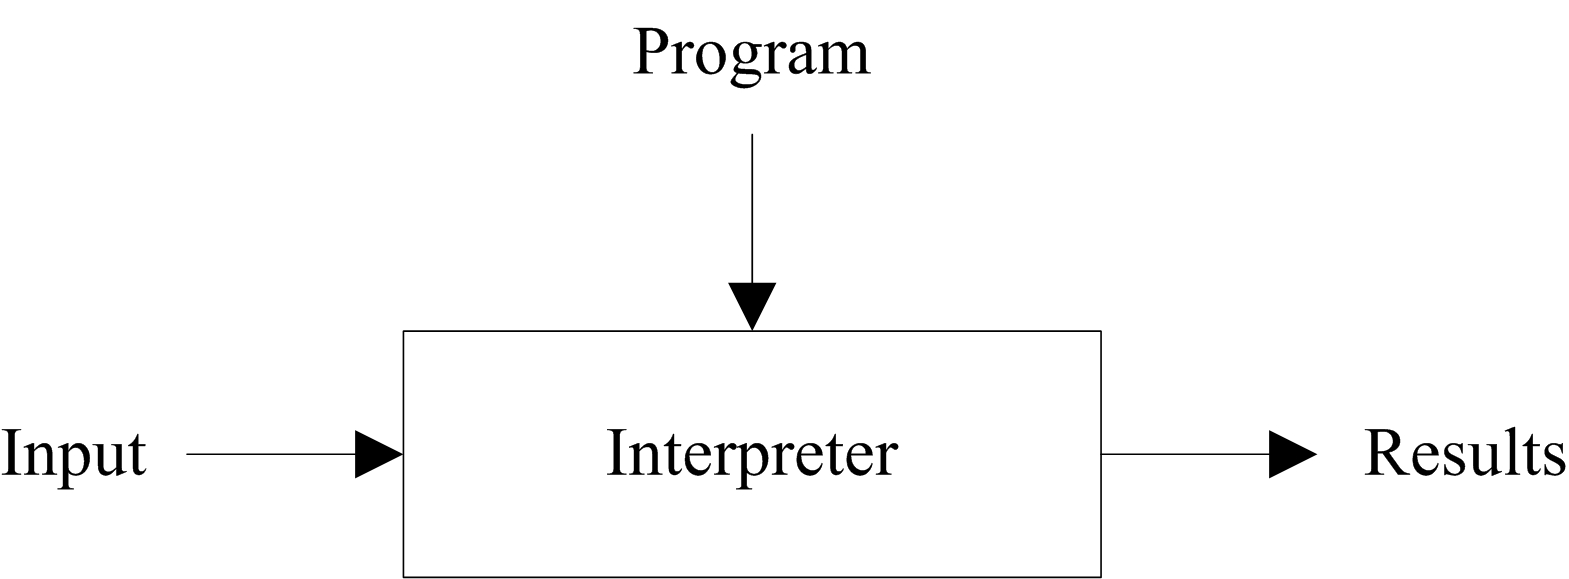
\includegraphics[scale=0.6]{{figures/figure01.02}.jpg}}
\end{center}

\pause
\bigskip

Examples of programming languages whose programs may be interpreted directly are the UNIX shell languages, such as bash and csh, Python, and many versions of LISP
\end{frame}

\section{Why Study Compilers?}
\begin{frame}[fragile]
\pause

Compilers are larger programs than the ones you have written in your programming courses

\pause
\bigskip

Compilers make use of all those things you have learned about earlier: arrays, lists, queues, stacks, trees, graphs, maps, regular expressions and finite state automata, context-free grammars and parsers, recursion and patterns

\pause
\bigskip

You learn a lot about the language you are compiling (in our case, Java)

\pause
\bigskip

You learn a lot about the target machine (in our case, both the Java Virtual Machine and the MIPS computer)

\pause
\bigskip

Compilers are still being written for new languages and targeted to new computer architectures

\pause
\bigskip

There is a good mix of theory and practice, and each is relevant to the other

\pause
\bigskip

The organization of a compiler is such that it can be written in stages, and each stage makes use of earlier stages; compiler writing is a case study in software engineering

\pause
\bigskip

Compilers are programs and writing programs is fun
\end{frame}

\section{The Phases of Compilation}
\begin{frame}[fragile]
\pause

At the very least, a compiler can be broken into a front end and a back end

\begin{center}
\visible<2->{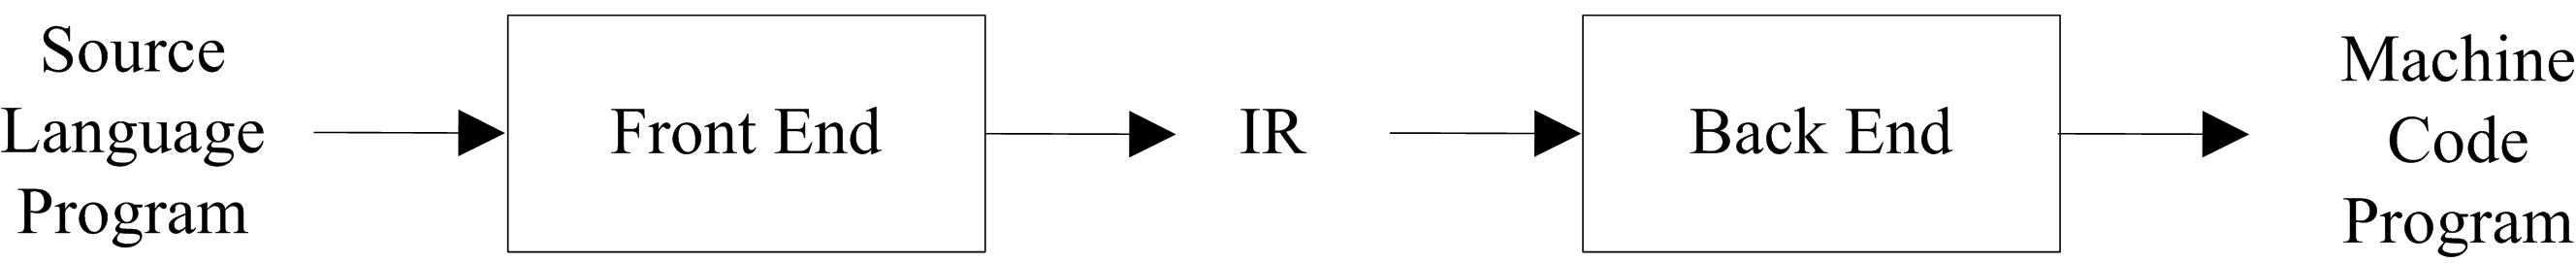
\includegraphics[scale=0.6]{{figures/figure01.03}.jpg}}
\end{center}

\pause
\bigskip

The front end takes as input, a high-level language program, and produces as output an intermediate representation (IR) of that program

\pause
\bigskip

The back end then takes the IR of the program as input, and produces the target machine language program
\end{frame}

\begin{frame}[fragile]
\pause

A compiler's front end analyzes the input program to determine its meaning, and so is source language dependent and target language independent

\pause
\bigskip

The front end can be further decomposed into a sequence of analysis phases

\begin{center}
\visible<3->{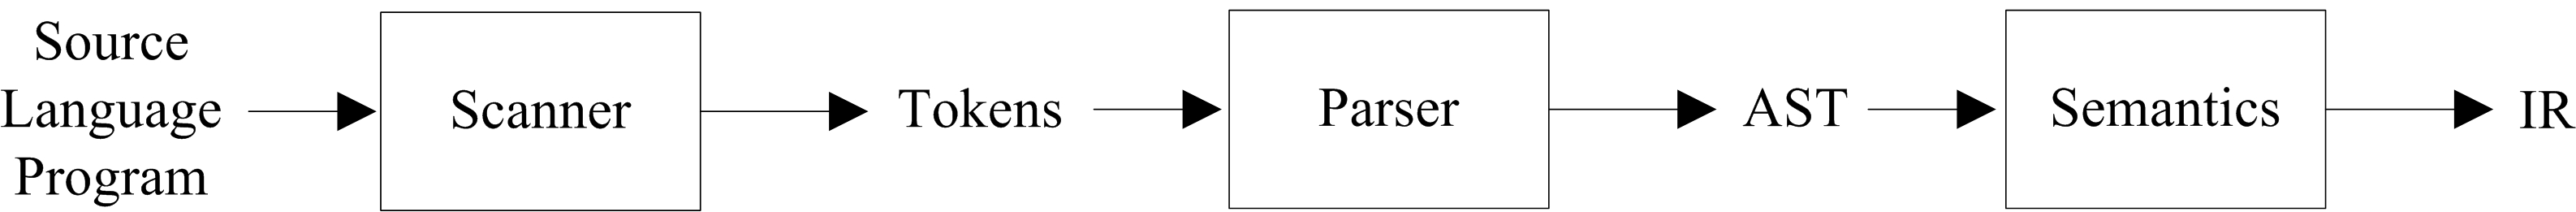
\includegraphics[scale=0.6]{{figures/figure01.04}.jpg}}
\end{center}

\pause
\bigskip

The scanner breaks the input stream of characters to a stream of tokens: identifiers, literals, reserved words, operators, and separators

\pause
\bigskip

The parser takes a sequence of tokens and parses it against a grammar to produce an abstract syntax tree (AST), which makes the syntax that is implicit in the source program, explicit

\pause
\bigskip

The semantics phase does semantic analysis: declares names in a symbol table, looks up names as they are referenced to determine their types, assigns types to expressions, and checks the validity of types; sometimes, a certain amount of storage analysis (such as assigning addresses or offsets to variables) is also done
\end{frame}

\begin{frame}[fragile]
\pause

A compiler's back end takes the IR and produces (synthesizes) a target machine program having the same meaning, and so is target language dependent and source language independent

\pause
\bigskip

The back end can be further decomposed into a sequence of synthesis phases

\begin{center}
\visible<3->{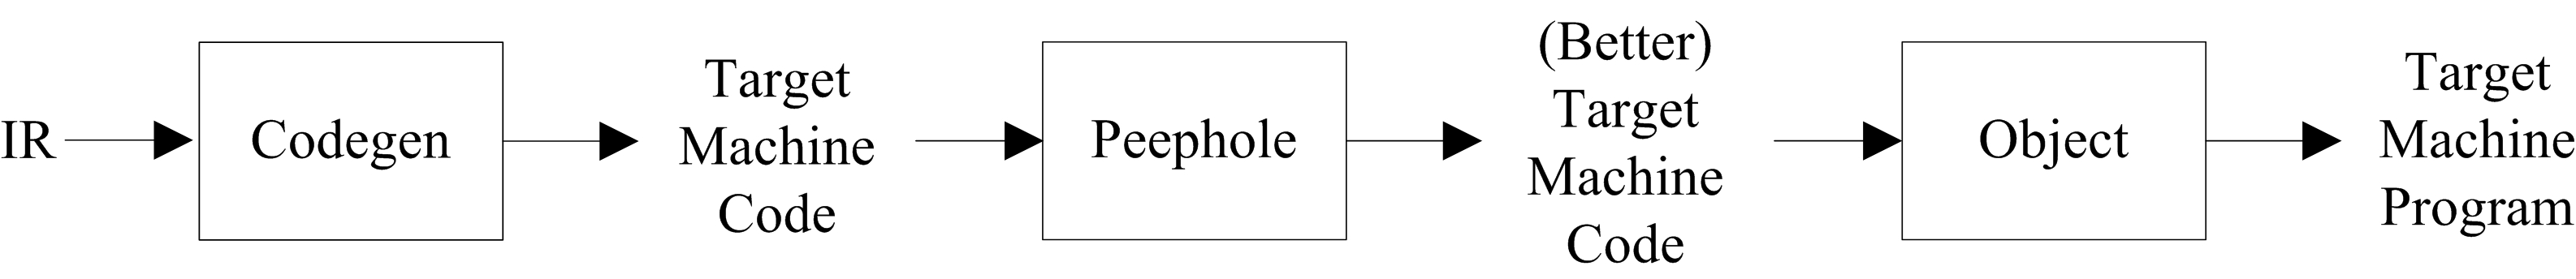
\includegraphics[scale=0.6]{{figures/figure01.05}.jpg}}
\end{center}

\pause
\bigskip

The code generation phase chooses what target machine instructions to generate, making use of information collected in earlier phases

\pause
\bigskip

The peephole phase scans through the generated instructions looking locally for wasteful instruction sequences such as branches to branches and unnecessary load/store pairs

\pause
\bigskip

The object phase links together any modules produced in code generation and it constructs a single machine code executable program
\end{frame}

\begin{frame}[fragile]
\pause

Sometimes, a compiler will have an optimizer (``middle end''), which sits between the front end and the back end

\begin{center}
\visible<2->{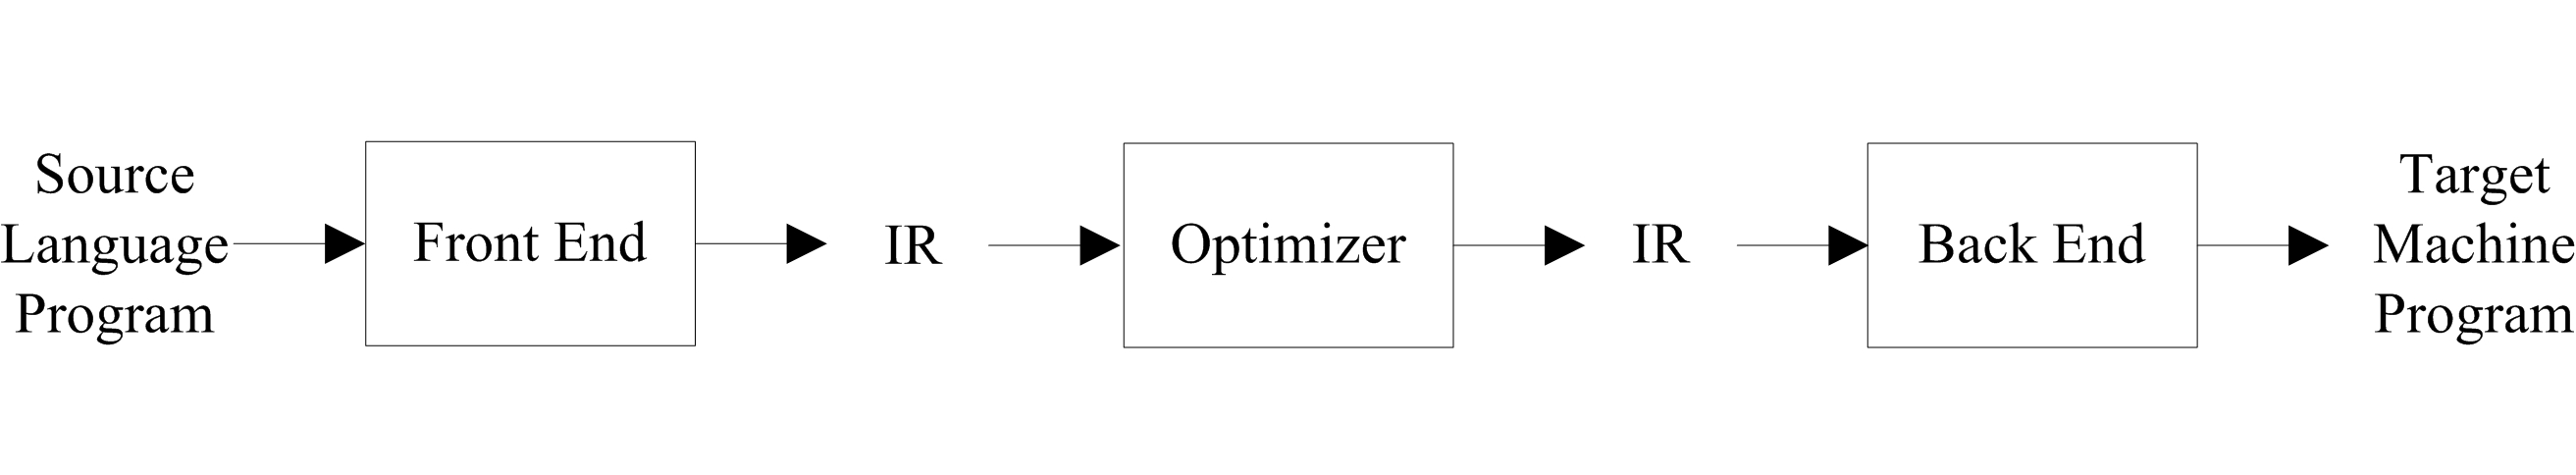
\includegraphics[scale=0.6]{{figures/figure01.06}.jpg}}
\end{center}

\pause
\bigskip

The purpose of the optimizer is both to improve the IR program and to collect information
that the back end may use for producing better code

\pause
\bigskip

The optimizer might do any number of the following
\begin{itemize}
\item Organize the program into what are called basic blocks: blocks of code from
which there are no branches out and into which there are no branches

\item From the basic block structure, one may then compute next-use information for determining the lifetimes of variables, and gather loop information

\item Next-use information is useful for eliminating common sub-expressions and constant folding (for example, replacing \lstinline{x + 5} by \lstinline{9} if we know \lstinline{x} has the value \lstinline{4})

\item Loop information is useful for pulling loop invariants out of loops and for strength reduction (for example, replacing multiplication operations by addition operations)
\end{itemize}
\end{frame}

\begin{frame}[fragile]
\pause

There are several advantages to separating the front end from the back end:
\begin{enumerate}
\item Decomposition reduces complexity; it's easier to understand (and implement) the smaller programs

\item Decomposition makes it possible for several individuals or teams to work concurrently on separate parts, reducing the overall implementation time

\item Decomposition permits a certain amount of code re-use; for example, once one has written
a front end for Java and a back end for the Intel Core Duo, one need only write a new C front end to get a C compiler, and one need only write a single SPARC back end to re-target both compilers to the SPARC architecture

\begin{center}
\visible<2->{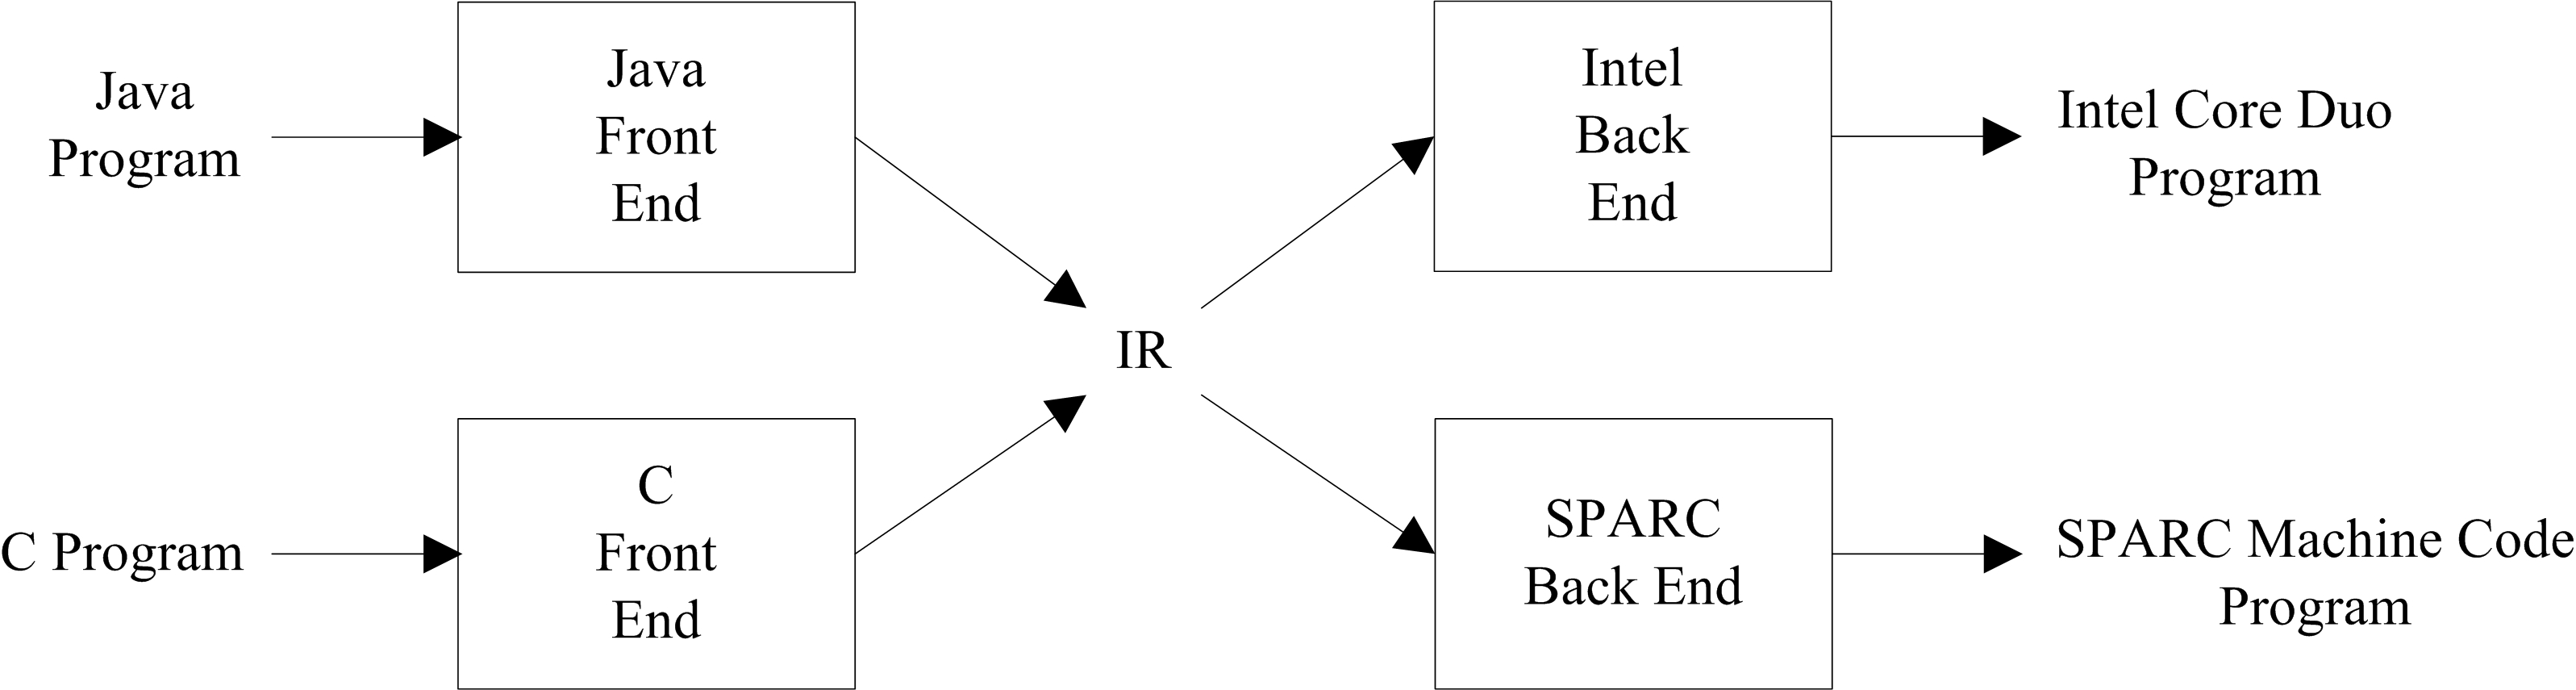
\includegraphics[scale=0.6]{{figures/figure01.07}.jpg}}
\end{center}
\end{enumerate}
\end{frame}

\begin{frame}[fragile]
\pause

The Java compiler, the program invoked when one types, for example
\begin{lstlisting}[language={}]
$ javac MyProgram.java
\end{lstlisting}
produces a \lstinline{MyProgram.class} file, a byte code program suitable for execution on the JVM

\pause
\bigskip

To execute the \lstinline{MyProgram.class} file, one types
\begin{lstlisting}[language={}]
$ java MyProgram
\end{lstlisting}
which effectively interprets the JVM program

\pause
\bigskip

In this course, we'll study the implementation of a compiler called \jmm to compile a (non-trivial) subset of Java, which we also call \jmm

\pause
\bigskip

In the first instance, we'll target the JVM

\pause
\bigskip

Targeting the JVM is deficient in one respect: one does not learn about register allocation because the JVM is a stack-based architecture and has no registers

\pause
\bigskip

To remedy this deficiency, we'll also study the compilation of JVM code to code for the MIPS machine, which is a register-based architecture; in doing this, we face the challenge of mapping possibly many variables to a limited number of fast registers
\end{frame}

\section{Overview of the \protect \jmm to JVM Compiler}
\begin{frame}[fragile]
\pause

Our source language, \jmm, is a proper subset of the Java programming language; it is an object-oriented programming language, supporting classes, methods, fields, message expressions, and a variety of
statements, expressions and primitive types

\pause
\bigskip

The \jmm compiler is organized in an object-oriented fashion

\begin{center}
\visible<3->{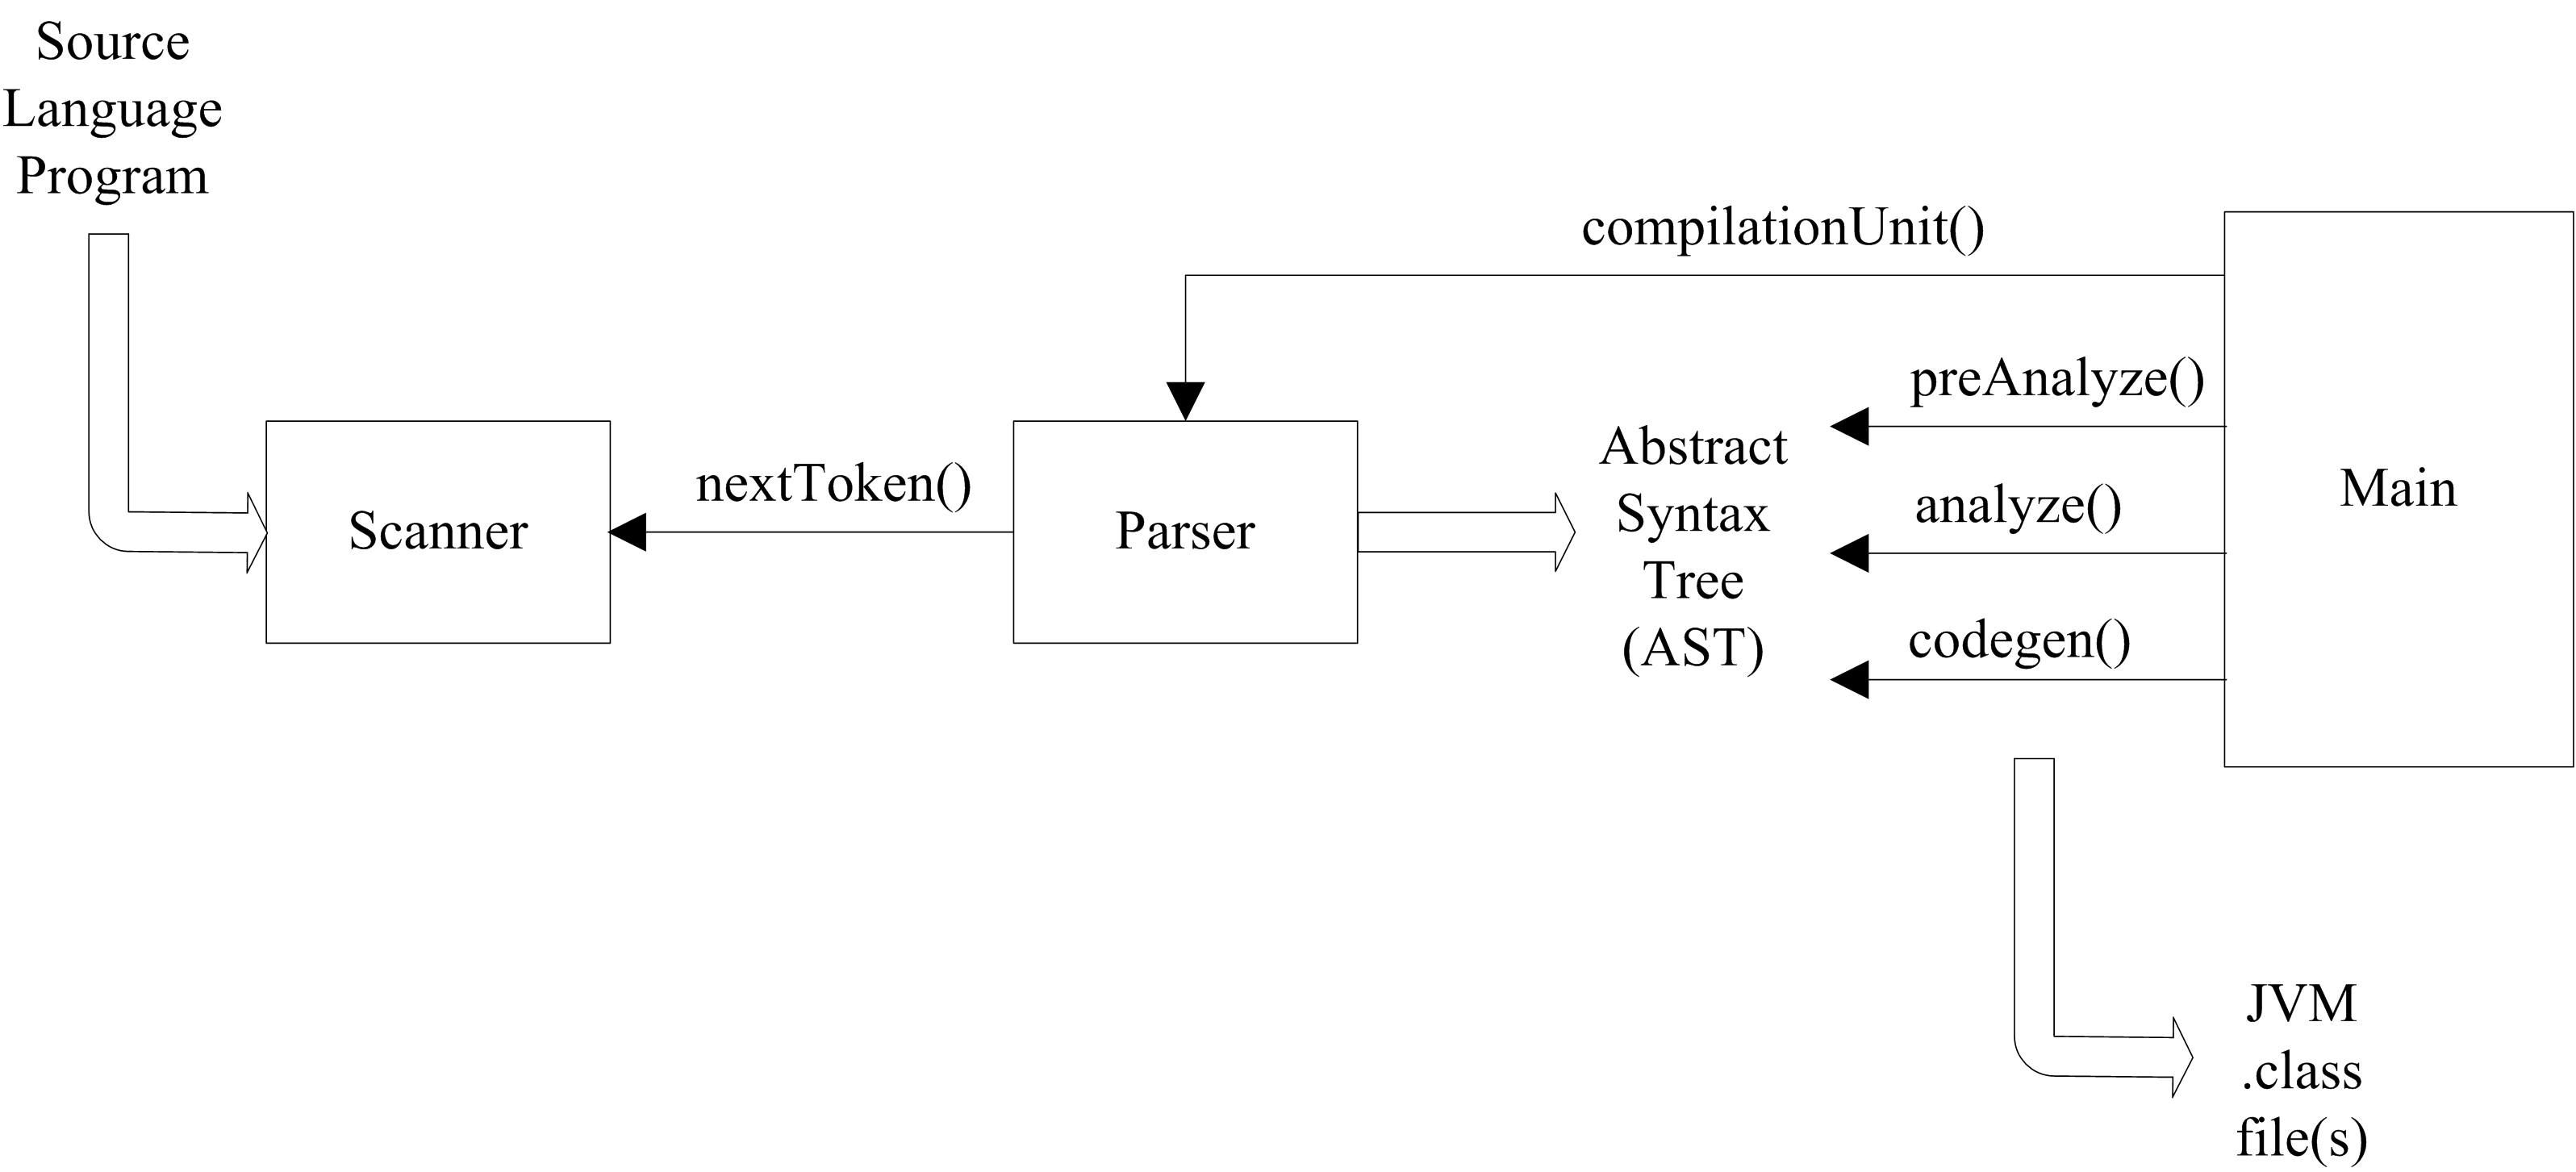
\includegraphics[scale=0.6]{{figures/figure01.08}.jpg}}
\end{center}
\end{frame}

\begin{frame}[fragile]
\pause

The scanner supports the parser, scanning tokens from the input stream of characters comprising the source language program

\pause
\bigskip

For example, the scanner breaks down the following source language \lstinline{HelloWorld} program

\begin{lstlisting}[language=Java]
import java.lang.System;

public class HelloWorld {
    // The only method.
    public static void main(String[] args) {
        System.out.println("Hello, World!");
    }
}
\end{lstlisting}

into atomic tokens such as \lstinline{import}, \lstinline{java}, \lstinline{.}, \lstinline{lang}, \lstinline{.}, \lstinline{System}, \lstinline{;}, and so on

\pause
\bigskip

Some tokens such as \lstinline{java}, \lstinline{HelloWorld}, and \lstinline{main} are \lstinline{IDENTIFIER} tokens, carrying along their images as attributes

\pause
\bigskip

Some tokens such as \lstinline{import}, \lstinline{public}, and \lstinline{class} are reserved words having the unique names such as \lstinline{IMPORT}, \lstinline{PUBLIC}, and \lstinline{CLASS}

\pause
\bigskip

Operators and separators such as \lstinline{+} and \lstinline{;} have distinct names such as \lstinline{PLUS} and \lstinline{SEMI}

\pause
\bigskip

Literals such as \lstinline{"Hello, World!"} comprise a single token such as \lstinline{STRING_LITERAL}

\pause
\bigskip

Comments are scanned and ignored altogether
\end{frame}

\begin{frame}[fragile]
\pause

The parsing of a \jmm program and the construction of its abstract syntax tree (AST) is driven by the language's syntax, and so is said to be syntax directed

\pause
\bigskip

In the first instance, our parser is hand-crafted from the \jmm grammar, to parse \jmm programs by a technique known as recursive descent

\pause
\bigskip

For example, consider the following grammatical rule describing the syntax for a compilation unit
\begin{lstlisting}[language={}]
compilationUnit ::= [PACKAGE qualifiedIdentifier SEMI]
                    {IMPORT  qualifiedIdentifier SEMI}
                    {typeDeclaration} EOF 
\end{lstlisting}

\pause
\bigskip

To parse a compilation unit using the recursive descent technique, one would write a method, call it \lstinline{compilationUnit()}

\begin{lstlisting}[language=Java]
    public JCompilationUnit compilationUnit() {
        int line = scanner.token().line();
        TypeName packageName = null; // Default
        if (have(PACKAGE)) {
            packageName = qualifiedIdentifier();
            mustBe(SEMI);
        }
\end{lstlisting}
\end{frame}

\begin{frame}[fragile]
\pause

\begin{lstlisting}[language=Java]
        ArrayList<TypeName> imports = new ArrayList<TypeName>();
        while (have(IMPORT)) {
            imports.add(qualifiedIdentifier());
            mustBe(SEMI);
        }
        ArrayList<JAST> typeDeclarations = new ArrayList<JAST>();
        while (!see(EOF)) {
            JAST typeDeclaration = typeDeclaration();
            if (typeDeclaration != null) {
                typeDeclarations.add(typeDeclaration);
            }
        }
        mustBe(EOF);
        return new JCompilationUnit(scanner.fileName(), line, packageName,
                imports, typeDeclarations);
    }
\end{lstlisting}
\end{frame}


\begin{frame}[fragile]
\pause

An AST for the \lstinline{HelloWorld} program

\begin{center}
\visible<2->{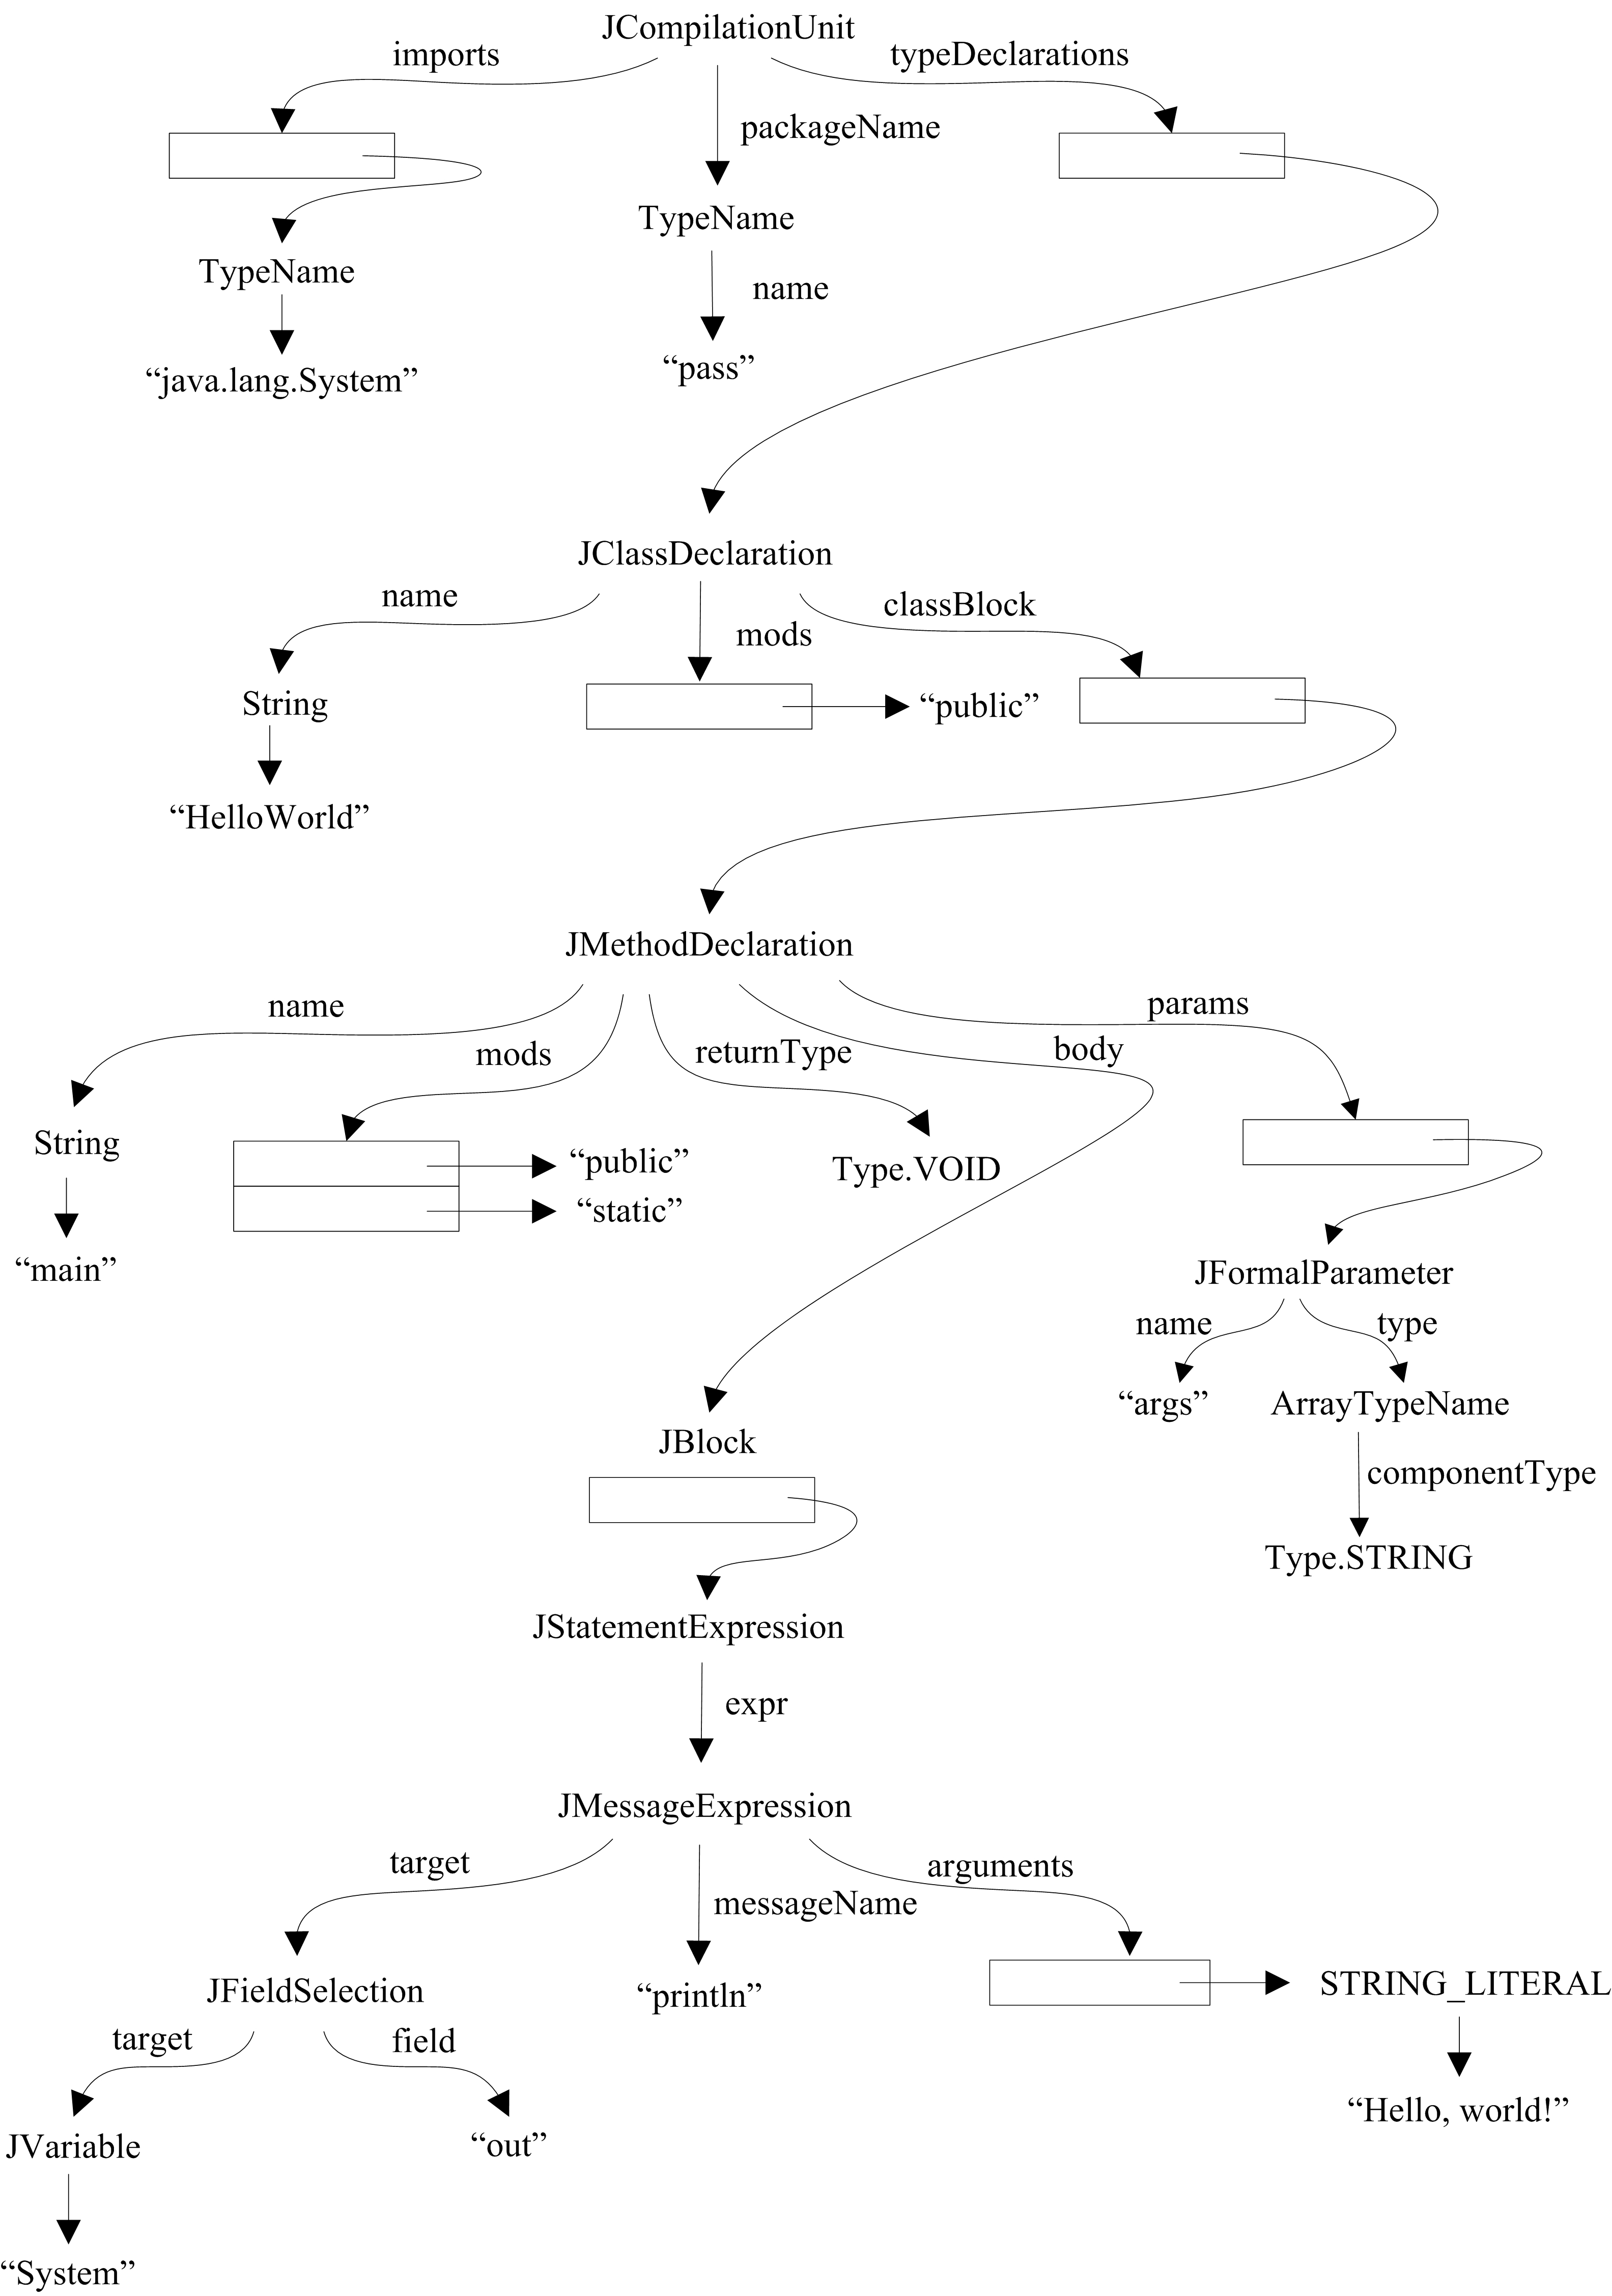
\includegraphics[scale=0.35]{{figures/figure01.09}.jpg}}
\end{center}
\end{frame}

\begin{frame}[fragile]
\pause

As in Java, \jmm names and values have types, and since \jmm (like Java) is statically typed, its compiler must determine the types of all names and expressions

\pause
\bigskip

Types in \jmm are represented using: \lstinline{Type} (wraps \lstinline{java.lang.Class}), \lstinline{Method} (wraps \lstinline{java.lang.reflect.Method}), \lstinline{Constructor} (wraps \lstinline{java.lang.reflect.Constructor}), \lstinline{Field} (wraps \lstinline{java.lang.reflect.Field}), and \lstinline{Member} (wraps \lstinline{java.lang.reflect.Member})

\pause
\bigskip

There are places where we want to denote a type by its name, before its type is known or defined, and for this we use \lstinline{TypeName} and (because we need array types) \lstinline{ArrayTypeName}

\pause
\bigskip

The \jmm compiler maintains a symbol table (a singly-linked list of \lstinline{Context} objects) in which it declares names; each object in the symbol table represents some area of scope and contains a mapping from names to definitions

\pause
\bigskip

A \lstinline{CompilationUnitContext} object represents the scope comprising the program, ie, the entire compilation unit

\pause
\bigskip

A \lstinline{ClassContext} object represents the scope of a class declaration

\pause
\bigskip

A \lstinline{LocalContext} object represents the scope of a block

\pause
\bigskip

A \lstinline{MethodContext} (subclass of \lstinline{LocalContext}) object represents the scopes of methods and, by extension, constructors
\end{frame}

\begin{frame}[fragile]
\pause

\lstinline{preAnalyze()} is a first pass at type checking, which builds that part of the symbol table that is at the top of the AST, to declare both imported types and types introduced by class declarations, and to declare the members in those classes

\pause
\bigskip

\lstinline{analyze()} picks up where \lstinline{preAnalyze()} left off and continues to build the symbol table, decorating the AST with type information and enforcing the \jmm type rules

\pause
\bigskip

\lstinline{analyze()} also performs other important tasks such as type checking, accessibility, member finding, tree rewriting, and storage allocation
\end{frame}

\begin{frame}[fragile]
\pause

The JVM is a stack machine: all computations are carried out atop the run-time stack

\pause
\bigskip

Each time a method is invoked, the JVM allocates a stack frame, a contiguous block of
memory locations on top of the run-time stack; the actual arguments substituted for formal parameters, the values of local variables, and temporary results are all given positions within this stack frame

\begin{center}
\visible<3->{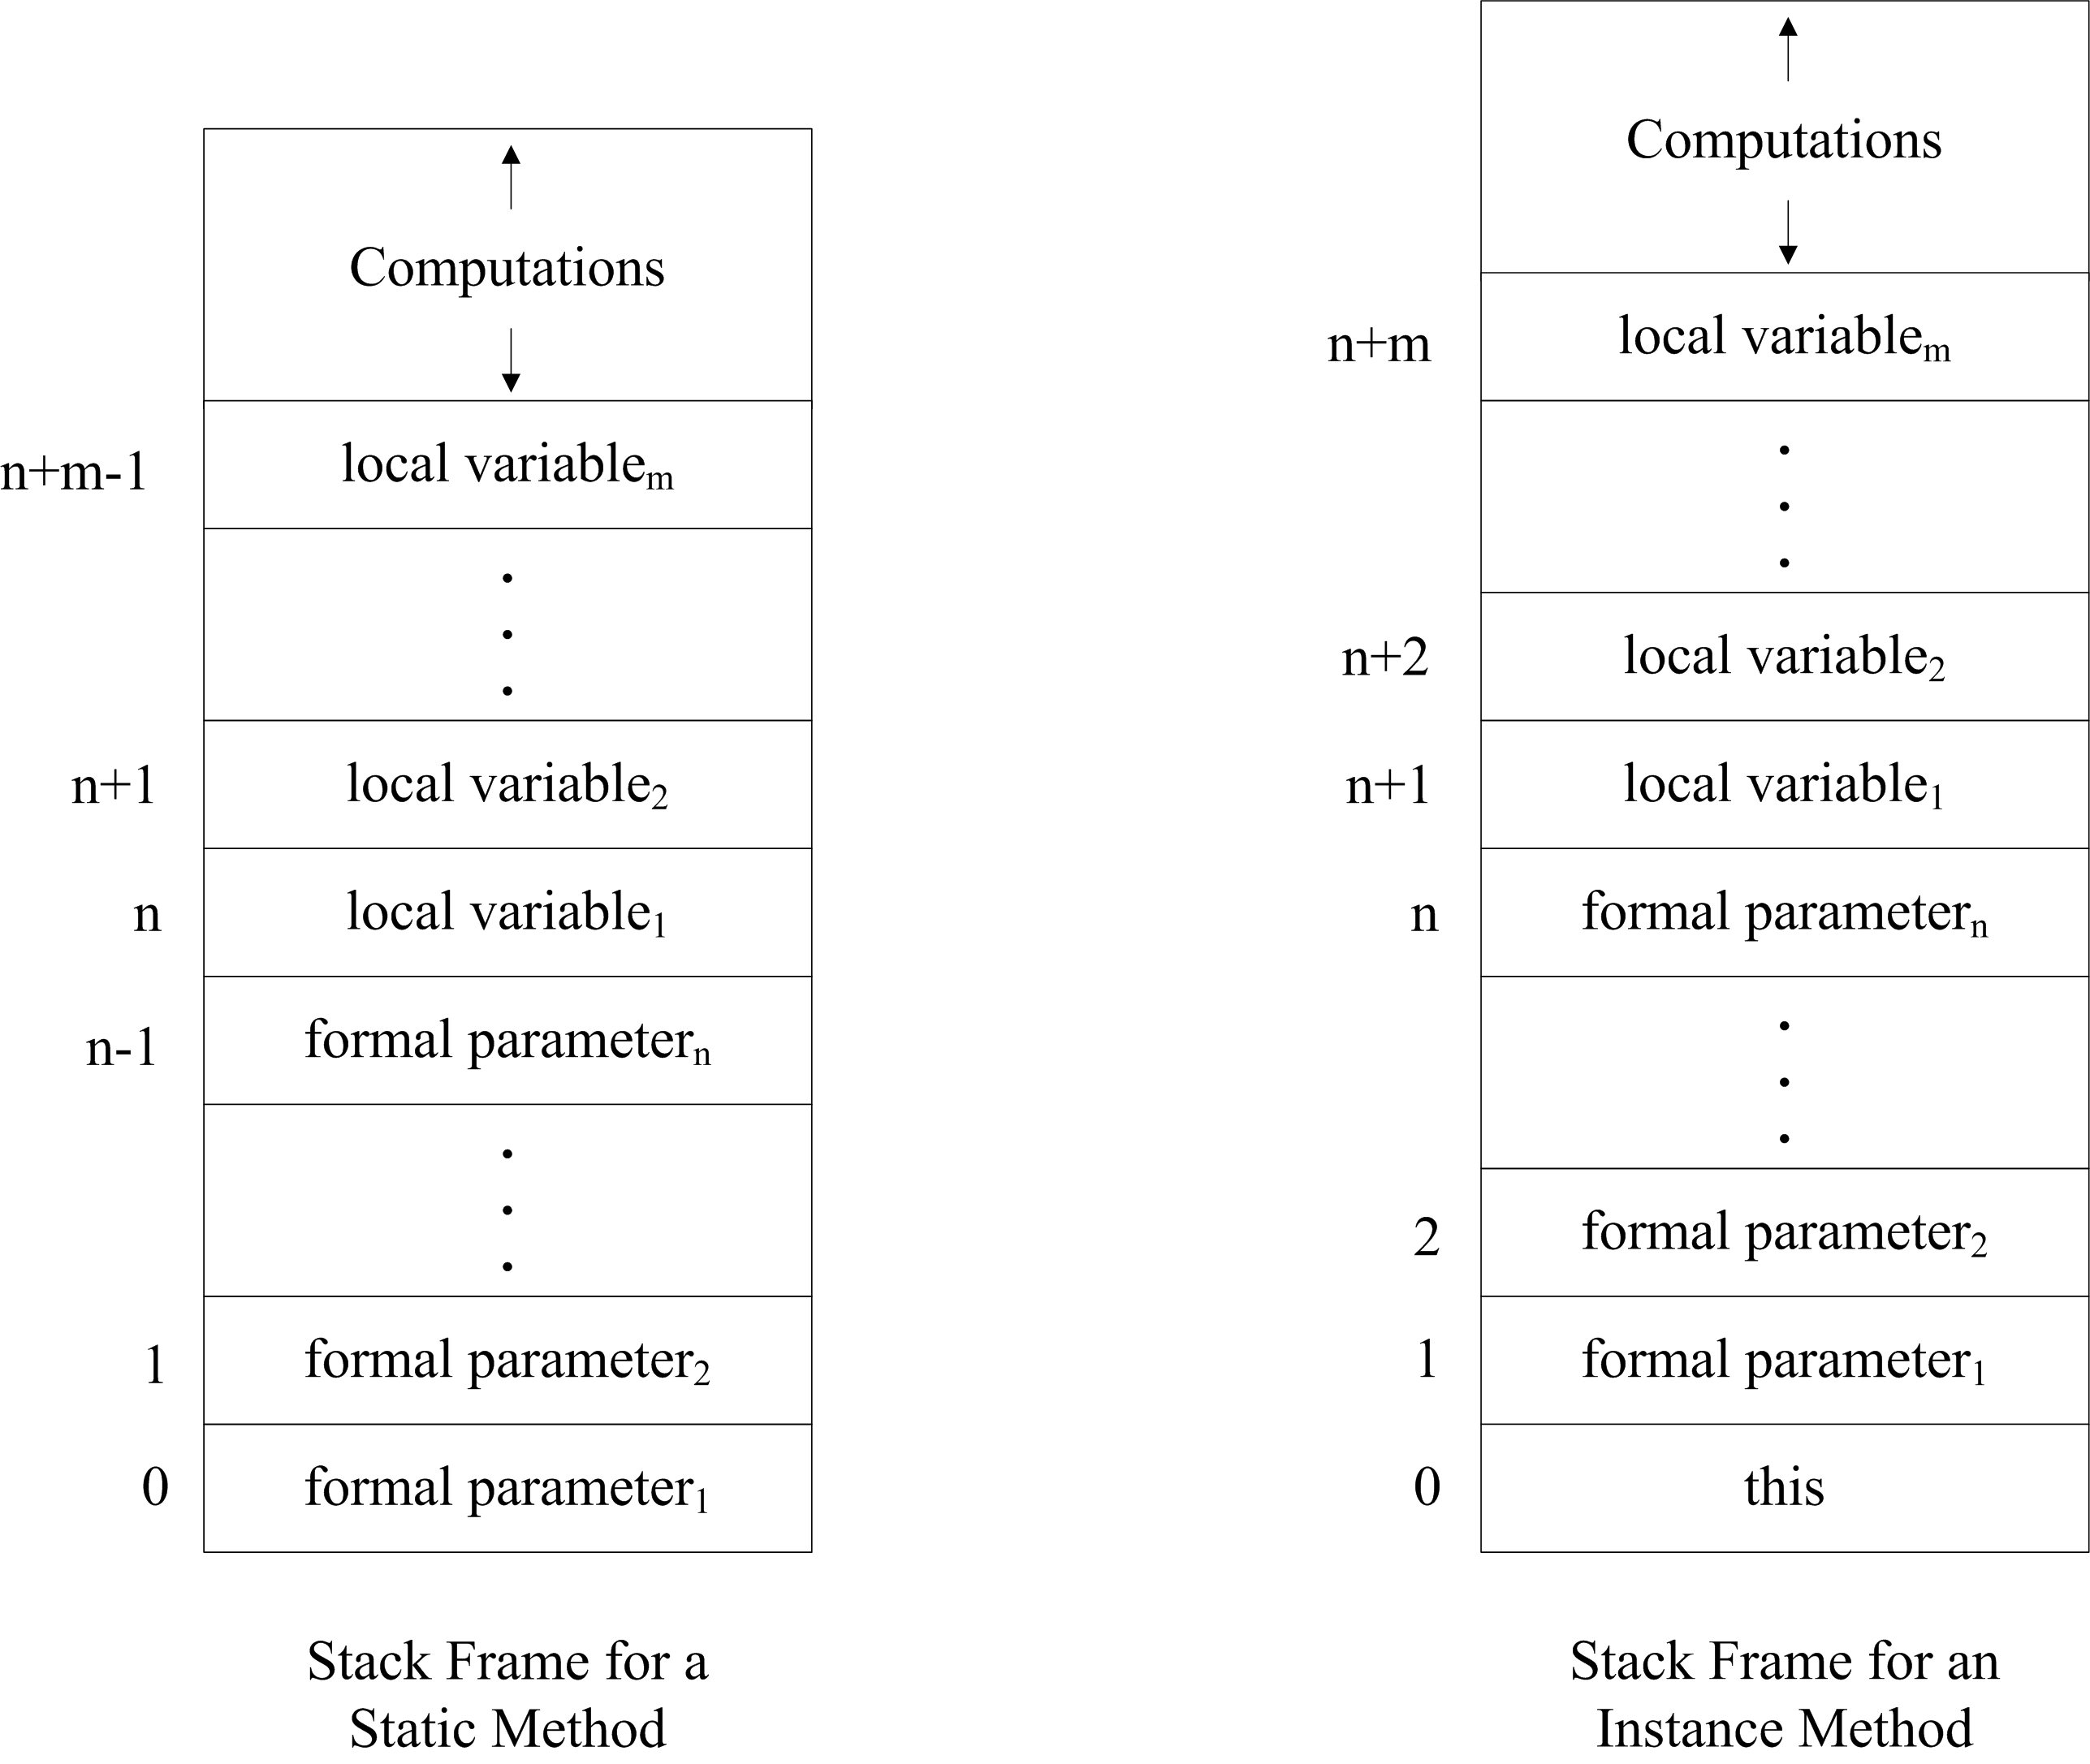
\includegraphics[scale=0.5]{{figures/figure01.10}.jpg}}
\end{center}
\end{frame}

\begin{frame}[fragile]
\pause

The purpose of \lstinline{codegen()} is to generate JVM byte code from the AST, based on information computed by \lstinline{preAnalyze()} and \lstinline{analyze()}

\pause
\bigskip

\lstinline{codegen()} is invoked by \lstinline{Main} on the root of the AST, and \lstinline{codegen()} recursively descends the AST, generating byte code

\pause
\bigskip

\lstinline{CLEmitter} provides an abstraction for the JVM class file, hiding many of the gory details

\pause
\bigskip

Here's the implementation of \lstinline{codegen()} in \lstinline{JMethodDeclaration} (AST representation for method declarations)

\begin{lstlisting}[language=Java]
    public void codegen(CLEmitter output) {
        output.addMethod(mods, name, descriptor, null, false);
        if (body != null) {
            body.codegen(output);
        }

        // Add implicit RETURN
        if (returnType == Type.VOID) {
            output.addNoArgInstruction(RETURN);
        }
    }
\end{lstlisting}
\end{frame}

\section{The \protect \jmm Compiler Source Tree}
\begin{frame}[fragile]
\pause

The zip file \lstinline{j--.zip} containing the \jmm distribution may be unzipped into any directory of your choosing; we refer to this directory as \lstinline{$j}

\pause
\bigskip

\lstinline{$j/j--/src/jminusminus} contains the source files for the compiler, where \lstinline{jminusminus} is a package, and these include
\begin{itemize}
\item \lstinline{Main.java}, the driver program
\item A hand-written scanner (\lstinline{Scanner.java}) and parser (\lstinline{Parser.java})
\item \lstinline{J*.java} files defining classes representing the AST nodes
\item \lstinline{CL*.java} files supplying the back-end code that is used by \jmm for creating JVM byte
code; the most important file amongst these is \lstinline{CLEmitter.java}, which provides the interface between the front end and back end of the compiler
\item \lstinline{S*.java} files that translate JVM code to SPIM files (SPIM is an interpreter for the
MIPS machine’s symbolic assembly language)
\item \lstinline{j--.jj}, the input file to JavaCC containing the specification for generating (as opposed to hand-writing) a scanner and parser for the \jmm language; \lstinline{JavaCCMain}, the driver program that uses the scanner and parser produced by JavaCC
\item Other Java files providing representation for types and the symbol table
\end{itemize}
\end{frame}

\begin{frame}[fragile]
\pause

\lstinline{$j/j--/bin/j--} is a script to run the compiler and has the following command-line
syntax
\begin{lstlisting}[language={}]
Usage: j-- <options> <source file>
where possible options include:
  -t Only tokenize input and print tokens to STDOUT
  -p Only parse input and print AST to STDOUT
  -pa Only parse and pre-analyze input and print AST to STDOUT
  -a Only parse, pre-analyze, and analyze input and print AST to STDOUT
  -s <naive|linear|graph> Generate SPIM code
  -r <num> Max. physical registers (1-18) available for allocation; default = 8
  -d <dir> Specify where to place output files; default = .
\end{lstlisting}

\pause
\bigskip

For example, the \jmm program \lstinline{$j/j--/tests/pass/HelloWorld.java} can be compiled
using \lstinline{j--} as follows

\begin{lstlisting}[language={}]
$ $j/j--/bin/j-- $j/j--/tests/pass/HelloWorld.java
\end{lstlisting}

to produce a \lstinline{HelloWorld.class} file under \lstinline{pass} folder within the current directory, which can then be run as

\begin{lstlisting}[language={}]
$ java pass.HelloWorld
\end{lstlisting}

to produce as output

\begin{lstlisting}[language={}]
$ Hello, World!
\end{lstlisting}
\end{frame}

\begin{frame}[fragile]
\pause

\jmm provides an elaborate framework with which one may add new Java constructs to the \jmm language

\pause
\bigskip

As an illustrative example, let's add the division operator to \jmm, which involves modifying the scanner to recognize \lstinline{/} as a token, modifying the parser to be able to parse division expressions, implementing semantic analysis, and finally, code generation for the division operation

\pause
\bigskip

Writing tests
\begin{itemize}
\item Place the following file (\lstinline{Division.java}) under \lstinline{$j/j--/tests/pass}

\begin{lstlisting}[language=Java]
package pass;

public class Division {
    public int divide(int x, int y) {
        return x / y ;
    }
}  
\end{lstlisting}
\end{itemize}
\end{frame}

\begin{frame}[fragile]
\pause

Writing tests (contd.)
\begin{itemize}
\item Place the following file (\lstinline{DivisionTest.java}) under \lstinline{$j/j--/tests/junit}

\begin{lstlisting}[language=Java]
public class DivisionTest extends TestCase {
    private Division division;

    protected void setUp() throws Exception {
        super.setUp();
        division = new Division();
    }

    protected void tearDown() throws Exception {
        super.tearDown();
    }

    public void testDivide() {
        this.assertEquals(division.divide(0, 42), 0);
        this.assertEquals(division.divide(42, 1), 42);
        this.assertEquals(division.divide(127, 3), 42);
    }
}
\end{lstlisting}

\item Make the following entry in the \lstinline{suite()} method of \lstinline{junit.JMinusMinusTestRunner}

\begin{lstlisting}[language=Java]
TestSuite suite = new TestSuite();
...
suite.addTestSuite(DivisionTest.class);
return suite;
\end{lstlisting}
\end{itemize}
\end{frame}

\begin{frame}[fragile]
\pause

Writing tests (contd.)
\begin{itemize}
\item Place the following file (\lstinline{Division.java}) under \lstinline{$j/j--/tests/fail}

\begin{lstlisting}[language=Java]
package fail;

import java.lang.System;

public class Division {
    public static void main(String[] args) {
        System.out.println('a' / 42);
    }
}
\end{lstlisting}
\end{itemize}

\pause
\bigskip

Changes to lexical and syntactic grammars
\begin{itemize}
\item Add a line describing the division operator to \lstinline{$j/j--/lexicalgrammar} under the operators section

\begin{lstlisting}[language={}]
DIV ::= "/"
\end{lstlisting}

\item Add a rule for the division operator to the rule describing multiplicative expressions in the \lstinline{$j/j--/grammar} file

\begin{lstlisting}[language={}]
multiplicativeExpression ::= unaryExpression // level 2
                               {(STAR | DIV) unaryExpression}
\end{lstlisting}
\end{itemize}
\end{frame}

\begin{frame}[fragile]
\pause

Changes to scanner
\begin{itemize}
\item Make the following change in \lstinline{TokenInfo}

\begin{lstlisting}[language=Java]
enum TokenKind {
    EOF (" < EOF >") ,
    ... ,
    STAR ("*") ,
    DIV ("/") ,
    ...
}
\end{lstlisting}

\item Make the following change in \lstinline{Scanner}

\begin{lstlisting}[language=Java]
if (ch == '/'’) {
    nextCh();
    if (ch == '/') {
        // CharReader maps all new lines to '\n'
        while (ch != '\n' && ch != EOFCH) {
            nextCh();
        }
    }
    else {
        return new TokenInfo(DIV, line);
    }
}
\end{lstlisting}
\end{itemize}
\end{frame}


\begin{frame}[fragile]
\pause

Changes to parser
\begin{itemize}
\item Define a class called \lstinline{JDivideOp} in \lstinline{JBinaryExpression.java} to represent an AST node for the division operator

\begin{lstlisting}[language=Java]
class JDivideOp extends JBinaryExpression {
    public JDivideOp(int line, JExpression lhs, JExpression rhs) {
        super(line, "/", lhs, rhs);
    }
    
    public JExpression analyze (Context context) { return this ; }
    
    public void codegen(CLEmitter output) { }
}
\end{lstlisting}

\item To parse expressions involving division operator, modify the \lstinline{multiplicativeExpression()} method in \lstinline{Parser.java} as follows

\begin{lstlisting}[language=Java]
private JExpression multiplicativeExpression() {
    int line = scanner.token().line();
    boolean more = true;
    JExpression lhs = unaryExpression();
    while (more) {
        if (have(STAR)) {
            lhs = new JMultiplyOp(line, lhs, unaryExpression());
        }
        else if (have(DIV)) {
            lhs = new JDivideOp(line, lhs, unaryExpression());
        }
        else { more = false; }
    }
    return lhs;
}
\end{lstlisting}
\end{itemize}
\end{frame}

\begin{frame}[fragile]
\pause

Semantic analysis and code generation
\begin{itemize}
\item Implement \lstinline{analyze()} in \lstinline{JDivideOp} as follows

\begin{lstlisting}[language=Java]
public JExpression analyze(Context context) {
    lhs = (JExpression) lhs.analyze(context);
    rhs = (JExpression) rhs.analyze(context);
    lhs.type().mustMatchExpected(line(), Type.INT);
    rhs.type().mustMatchExpected(line(), Type.INT);
    type = Type.INT;
    return this;
}
\end{lstlisting}

\item Implement \lstinline{codegen()} in \lstinline{JDivideOp} as follows

\begin{lstlisting}[language=Java]
public void codegen(CLEmitter output) {
    lhs.codegen(output);
    rhs.codegen(output);
    output.addNoArgInstruction(IDIV);
}
\end{lstlisting}
\end{itemize}

\pause
\bigskip

To test the changes, run the following command inside the \lstinline{$j} directory

\begin{lstlisting}[language=Java]
$ ant
\end{lstlisting}
\end{frame}
\end{document}
